\def\figpath{tex/4_Konstantstromquelle/pictures}
\graphicspath{{tex/4_Konstantstromquelle/pictures/}}

\chapter{Konstantstromquelle}
In Kapitel 4 wird die Auslegung einer Konstantstromquelle, welche mittels Bipolartransistoren realisiert wird, behandelt. Im folgenden wird auf die Berechnung, die Simulation und das Temperaturverhalten der Schaltung eingegangen. 

\section{Wahl der Stromquellenschaltung und Auslegung der Widerstände}
Für die zu untersuchende Stromquelle wird die Schaltung eines einfachen Stromspiegels gewählt, siehe Abb. \ref{fig_Kap4_01:Stromspiegel01}. 

\begin{figure}[H]
	\centering
	\def\svgwidth{0.5\textwidth}
	\input{\figpath/EinfacherStromspiegel.pdf_tex}
	\caption{Einfache Stromspiegelschaltung} 
	\label{fig_Kap4_01:Stromspiegel01} 
\end{figure}

Die Transistoren $T_1$ und $T_2$ werden baugleich gewählt (jeweils Typ BC547B), womit auch 
\begin{equation}
    B_1 = B_2 = B
\end{equation}
gelten soll. 

Des weiteren gilt für den Kollektorstrom an einem npn-Bipolartransistor

\begin{equation}
    \label{glgn_transist}
    I_C = I_S \left(e^{\frac{U_{BE}}{U_T}} - 1 \right) .
\end{equation}

Für Masche I aus Abb. \ref{fig_Kap4_01:Stromspiegel01} gilt

\begin{equation}
    \text{MI: } U_{BE,1} + I_{C,1}\left( 1 + \frac{1}{B}\right)R_{E,1} = U_{BE,2} + I_{C,2}\left( 1 + \frac{1}{B}\right)R_{E,2} .
\end{equation}

Wählt man beide Emitterwiderstände gleich groß, so ergibt sich die Gleichung

\begin{equation}
    U_{BE,1} + I_S \left(e^{\frac{U_{BE,1}}{U_T}} - 1 \right)\left( 1 + \frac{1}{B}\right)R_E = U_{BE,2} + I_S \left(e^{\frac{U_{BE,2}}{U_T}} - 1 \right)\left( 1 + \frac{1}{B}\right)R_E .
    \label{glng_transzend}
\end{equation}

Es ist naheliegend, dass sich durch den symmetrischen Schaltungsaufbau als Lösung der transzendenten Gleichung \ref{glng_transzend} wiederum gleich große Basis-Emitterspannungen einstellen werden, 

\begin{equation}
    U_{BE,1} = U_{BE,2} .
\end{equation}

Aus Gleichung \ref{glgn_transist} folg somit
\begin{equation}
    I_{C,1} = I_{C,2} = I_C \quad \Rightarrow \quad I_{B,1} = I_{B,2} = I_B
\end{equation}

Mithilfe von Knoten I erhält man die Gleichung

\begin{equation}
    I_e = I_C + 2 \cdot I_B = I_C \cdot \left( 1 + \frac{2}{B} \right) .
\end{equation}

Daraus lässt sich ein Zusammenhang zwischen Referenzstrom $I_e$ und Ausgangsstrom $I_a$ finden, 

\begin{equation}
    I_C = I_a = \frac{1}{1 + \frac{2}{B}} \cdot I_e  = k_I \cdot I_e .
\end{equation}

Aus Masche II ergibt sich folgender Zusammenhang

\begin{equation}
    U_B = U_{BE} + I_e \cdot R_1 + I_a \cdot \left(1 + \frac{1}{B} \right) \cdot R_E = U_{BE} + I_e \cdot \left( R_1 + k_I \left(1 + \frac{1}{B} \right) \cdot R_E \right) .
\end{equation}

Der Ausgangsstrom lässt sich daher folgendermaßen ausdrücken

\begin{equation}
    I_a = k_I I_e = k_I \frac{U_B - U_{BE}}{R_1 + k_I \left(1 + \frac{1}{B} \right) \cdot R_E} .
\end{equation}

Will man nun einen Ausgangsstrom von 

\begin{equation*}
    I_a = \SI{10}{\milli\ampere}
\end{equation*}

bei gegebenen Bauteilwerten (siehe Tab. \ref{tab_Kap4_01:Bauteilwerte} ) so ergibt sich für den Widerstand $R_1$

\begin{equation}
    R_1 = k_I \cdot \left(\frac{U_B - U_{BE}}{I_a} - R_1 \cdot \left( \right)\right) = \frac{1}{1+\frac{2}{290}}\left(\frac{\SI{15}{\volt} - \SI{0.7}{\volt}}{\SI{10}{\milli\ampere}} - \SI{100}{\ohm} \cdot \left( 1 + \frac{1}{290} \right)\right) = \SI{1.32}{\kilo\ohm} .
\end{equation}

\begin{table}[H]
\centering
\begin{tabular}{|c|c|} \hline
Benennung & Größe \\ \hline
$U_B$ & \SI{15}{\volt} \\ \hline
$B$ & 290 \\ \hline
$R_E$ & \SI{100}{\ohm} \\ \hline
\end{tabular}
\caption{Parameter für Berechnung und Simulation}
\label{tab_Kap4_01:Bauteilwerte} 
\end{table}

Die Gleichstromverstärkung $B$ wurde dem Datenblatt bei $I_C = \SI{2}{\milli\ampere}$ und $U_{CE} = \SI{5}{\volt}$ entnommen.

Von einer Konstantstromquelle darf eine gewisse Präzision erwartet werden, womit der Widerstand entsprechend der E48-Reihe mit

\begin{equation*}
    R_1 = \SI{1.33}{\kilo\ohm}
\end{equation*}

dimensioniert werden kann.

\section{Maximaler Lastwiderstand $R_{L,max}$}
Aus dem Datenblatt des BC547B lässt sich bei $I_C = \SI{10}{\milli\ampere}$ eine Kollektor-Emitter-Sättigungsspannung von 

\begin{equation}
    U_{CE,sat} = \SI{0.09}{\volt}
\end{equation}

ablesen.

Legt man eine Masche über die Ausgangsseite, ergibt sich

\begin{equation}
    U_B = R_{L,max} \cdot I_a + U_{CE,sat} + R_E \cdot I_a \cdot \left(1 + \frac{1}{B} \right) .
\end{equation}

Somit beträgt der maximale Lastwiderstand, ab der der Kollektorstrom einbricht

\begin{equation}
    R_{L,max} = \frac{U_B - U_{CE,sat}}{I_a} - R_E = \frac{\SI{15}{\volt} - \SI{0.09}{\volt}}{\SI{10}{\milli\ampere}} - \SI{100}{\ohm} = \SI{1.39}{\kilo\ohm} .
\end{equation}

\section{Strom in Abhängigkeit des Lastwiderstandes $I_a(R_L)$}
Für die LTSpice-Simulation wurde das Schematic aus Abb. \ref{fig_Kap4_02:SpiceSchematic} verwendet. 

\begin{figure}[H]
    \centering
    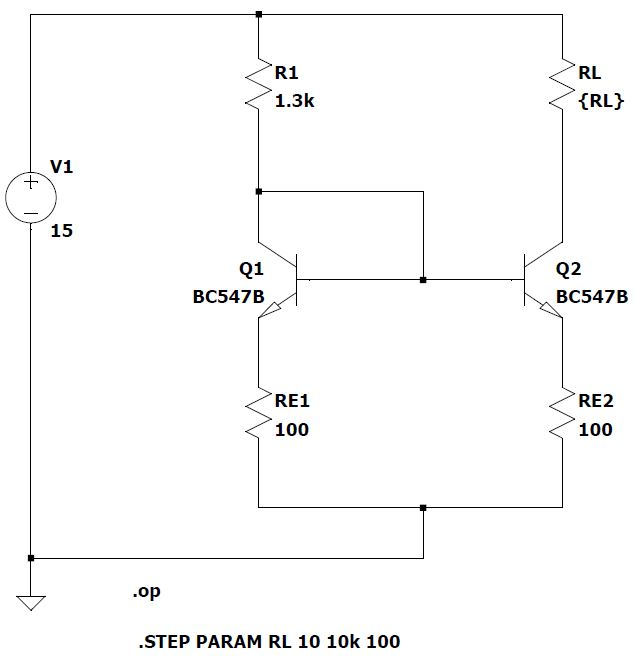
\includegraphics[width = 0.6\textwidth]{\figpath/einfacherStromspiegel.jpg}
    \caption{Einfacher Stromspiegel in LTSpice}
    \label{fig_Kap4_02:SpiceSchematic}
\end{figure}

Das Simulationsergebnis kann in Abb. \ref{fig_Kap4_03:Ia} betrachtet werden.

\begin{figure}[H]
	\centering \small
	\scalebox{0.9}{% This file was created by matlab2tikz.
%
\definecolor{mycolor1}{rgb}{0.00000,0.44700,0.74100}%
%
\begin{tikzpicture}

\begin{axis}[%
width=4.521in,
height=3.566in,
at={(0.758in,0.481in)},
scale only axis,
xmin=0,
xmax=10,
xlabel style={font=\color{white!15!black}},
xlabel={$R_L \text{ in k} \Omega$},
ymin=1,
ymax=11,
ylabel style={font=\color{white!15!black}},
ylabel={$I \text{ in mA}$},
axis background/.style={fill=white},
title style={font=\bfseries},
title={$I_a(R_L)$},
xmajorgrids,
ymajorgrids
]
\addplot [color=mycolor1, forget plot]
  table[row sep=crcr]{%
0.01	10.2021\\
0.11	10.19756\\
0.21	10.19295\\
0.31	10.18826\\
0.41	10.18349\\
0.51	10.17864\\
0.61	10.17371\\
0.71	10.16869\\
0.81	10.16358\\
0.91	10.15837\\
1.01	10.15307\\
1.11	10.14766\\
1.21	10.14216\\
1.31	10.13654\\
1.41	9.866105\\
1.51	9.252984\\
1.61	8.702559\\
1.71	8.211943\\
1.81	7.772927\\
1.91	7.378082\\
2.01	7.021202\\
2.11	6.697128\\
2.21	6.40157\\
2.31	6.130943\\
2.41	5.882232\\
2.51	5.652887\\
2.61	5.440736\\
2.71	5.243917\\
2.81	5.060831\\
2.91	4.89009\\
3.01	4.730487\\
3.11	4.580967\\
3.21	4.440606\\
3.31	4.308587\\
3.41	4.184188\\
3.51	4.066769\\
3.61	3.955759\\
3.71	3.850646\\
3.81	3.750974\\
3.91	3.65633\\
4.01	3.566343\\
4.11	3.480679\\
4.21	3.399033\\
4.31	3.321129\\
4.41	3.246716\\
4.51	3.175563\\
4.61	3.107462\\
4.71	3.04222\\
4.81	2.979661\\
4.91	2.919623\\
5.01	2.861956\\
5.11	2.806523\\
5.21	2.753197\\
5.31	2.701858\\
5.41	2.6524\\
5.51	2.604719\\
5.61	2.558722\\
5.71	2.514322\\
5.81	2.471435\\
5.91	2.429988\\
6.01	2.389907\\
6.11	2.351127\\
6.21	2.313586\\
6.31	2.277225\\
6.41	2.241988\\
6.51	2.207826\\
6.61	2.174689\\
6.71	2.142532\\
6.81	2.111312\\
6.91	2.080988\\
7.01	2.051524\\
7.11	2.022882\\
7.21	1.995029\\
7.31	1.967932\\
7.41	1.941562\\
7.51	1.915889\\
7.61	1.890886\\
7.71	1.866527\\
7.81	1.842788\\
7.91	1.819645\\
8.01	1.797076\\
8.11	1.77506\\
8.21	1.753577\\
8.31	1.732607\\
8.41	1.712134\\
8.51	1.692138\\
8.61	1.672604\\
8.71	1.653516\\
8.81	1.634859\\
8.91	1.616618\\
9.01	1.59878\\
9.11	1.581331\\
9.21	1.564258\\
9.31	1.547551\\
9.41	1.531196\\
9.51	1.515184\\
9.61	1.499503\\
9.71	1.484143\\
9.81	1.469095\\
9.91	1.454349\\
10	1.441328\\
};
\end{axis}
\end{tikzpicture}%}
	\caption{Ausgangsstrom in Abhängigkeit des Lastwiderstandes}
	\label{fig_Kap4_03:Ia}
\end{figure}

Man erkennt, dass der Ausgangsstrom bei ca. $\SI{1,4}{\kilo\ohm}$ einbricht, was gut mit den Berechnungen, siehe Glng. 4.14, übereinstimmt. Bis dahin fällt der Ausgangsstrom leicht, was durch den realen Innenwiderstand der Stromquelle begründet werden kann.

\section{Verlauf des Innenwiderstandes $R_i$}
Der Ausgangswiderstand des Stromspiegels entspricht dem Innenwiderstand der damit realisierten Stromquelle, womit gilt:

\begin{equation}
    r_a = \frac{\partial U_a}{\partial I_a}\big|_{I_e = const} \hat{=} R_i .
\end{equation}

Lt. Abb. \ref{fig_Kap4_04:Ri} wird nun am Ausgang der Lastwiderstand durch eine Spannungsquelle ersetzt und ein DC-Sweep durchgeführt. Die invertierte Ableitung des Kollektorstroms nach der Ausgangsspannung entspricht dem Verlauf des Innenwiderstandes, siehe Abb. \ref{fig_Kap4_05:Ri}.

\begin{figure}[H]
    \centering
    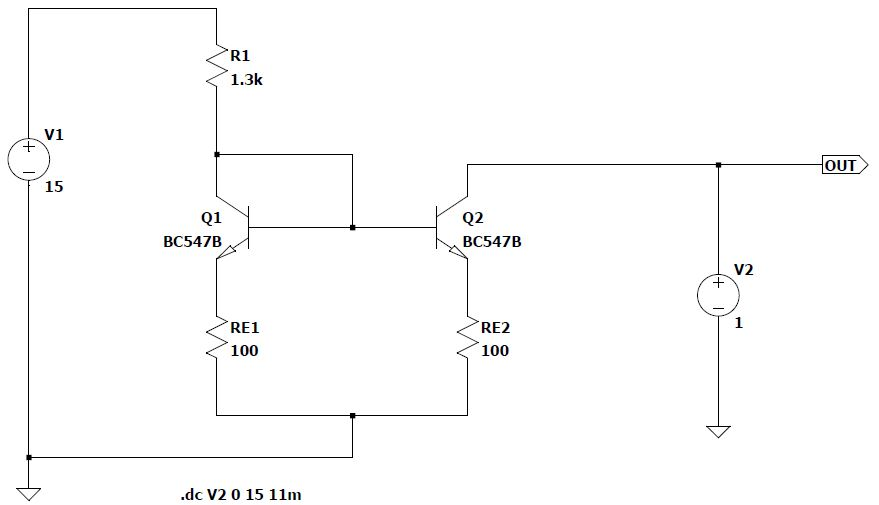
\includegraphics[width = 0.6\textwidth]{\figpath/stromspiegel_02.jpg}
    \caption{Schaltung zur Bestimmung des Innenwiderstandes}
    \label{fig_Kap4_04:Ri}
\end{figure}

\begin{figure}[H]
	\centering \small
	\scalebox{0.9}{% This file was created by matlab2tikz.
%
\definecolor{mycolor1}{rgb}{0.00000,0.44700,0.74100}%
%
\begin{tikzpicture}

\begin{axis}[%
width=4.521in,
height=3.566in,
at={(0.758in,0.481in)},
scale only axis,
xmin=0,
xmax=15,
xlabel style={font=\color{white!15!black}},
xlabel={$V_2 \text{ in V}$},
ymin=0,
ymax=250,
ylabel style={font=\color{white!15!black}},
ylabel={$R_i \text{ in k}\Omega$},
axis background/.style={fill=white},
title style={font=\bfseries},
title={$R_i(U_a)$},
xmajorgrids,
ymajorgrids
]
\addplot [color=mycolor1, forget plot]
  table[row sep=crcr]{%
0	0.0542671\\
0.05	0.05387898\\
0.1	0.05324937\\
0.15	0.05284118\\
0.2	0.0525694\\
0.25	0.05238921\\
0.3	0.05227581\\
0.35	0.05221523\\
0.4	0.0522001\\
0.45	0.05222774\\
0.5	0.05229935\\
0.55	0.05242011\\
0.6	0.05260025\\
0.65	0.05285732\\
0.7	0.05322076\\
0.75	0.0537411\\
0.8	0.05450972\\
0.85	0.05570508\\
0.9	0.0577147\\
0.95	0.0615101\\
1	0.0700162\\
1.05	0.09368813\\
1.1	0.1737182\\
1.15	0.5212997\\
1.2	2.494\\
1.25	13.83153\\
1.3	60.08628\\
1.35	132.8888\\
1.4	166.9894\\
1.45	174.8765\\
1.5	176.3123\\
1.55	176.6023\\
1.6	176.8932\\
1.65	177.1851\\
1.7	177.478\\
1.75	177.478\\
1.8	177.7718\\
1.85	178.0666\\
1.9	178.0666\\
1.95	178.3624\\
2	178.3624\\
2.05	178.6592\\
2.1	178.957\\
2.15	178.957\\
2.2	179.2557\\
2.25	179.5555\\
2.3	179.5555\\
2.35	179.5555\\
2.4	179.8563\\
2.45	180.158\\
2.5	180.4608\\
2.55	180.7646\\
2.6	180.7646\\
2.65	180.7646\\
2.7	181.0694\\
2.75	181.3753\\
2.8	181.3753\\
2.85	181.3753\\
2.9	181.6822\\
2.95	181.9901\\
3	182.2991\\
3.05	182.6092\\
3.1	182.6092\\
3.15	182.6092\\
3.2	182.9202\\
3.25	183.2324\\
3.3	183.2324\\
3.35	183.5456\\
3.4	183.5456\\
3.45	183.8599\\
3.5	184.1753\\
3.54999999999999	184.1753\\
3.6	184.4917\\
3.65	184.4917\\
3.69999999999999	184.8093\\
3.75	185.1279\\
3.79999999999999	185.1279\\
3.84999999999999	185.1279\\
3.89999999999999	185.4476\\
3.94999999999999	185.7685\\
3.99999999999999	186.0904\\
4.04999999999999	186.0904\\
4.09999999999999	186.0904\\
4.14999999999999	186.4135\\
4.19999999999999	186.7377\\
4.24999999999999	187.063\\
4.29999999999999	187.063\\
4.34999999999999	187.063\\
4.39999999999999	187.3895\\
4.44999999999999	187.7171\\
4.49999999999999	187.7171\\
4.54999999999999	187.7171\\
4.59999999999999	188.0459\\
4.64999999999999	188.3758\\
4.69999999999999	188.7068\\
4.74999999999999	188.7068\\
4.79999999999999	188.7068\\
4.84999999999999	189.0391\\
4.89999999999999	189.3725\\
4.94999999999999	189.3725\\
4.99999999999999	189.3725\\
5.04999999999999	190.0428\\
5.09999999999999	190.0428\\
5.14999999999999	190.0428\\
5.19999999999999	190.3798\\
5.24999999999999	190.7179\\
5.29999999999999	190.7179\\
5.34999999999999	190.7179\\
5.39999999999999	191.0573\\
5.44999999999999	191.3978\\
5.49999999999999	191.7396\\
5.54999999999999	191.7396\\
5.59999999999999	191.7396\\
5.64999999999999	192.0826\\
5.69999999999999	192.0826\\
5.74999999999999	192.4269\\
5.79999999999999	192.7723\\
5.84999999999999	192.7723\\
5.89999999999999	193.119\\
5.94999999999999	193.119\\
5.99999999999999	193.119\\
6.04999999999999	193.467\\
6.09999999999999	193.8162\\
6.14999999999999	193.8162\\
6.19999999999999	194.1667\\
6.24999999999999	194.5184\\
6.29999999999999	194.5184\\
6.34999999999999	194.5184\\
6.39999999999999	194.5184\\
6.44999999999999	194.8715\\
6.49999999999998	195.2258\\
6.54999999999998	195.5814\\
6.59999999999999	195.5814\\
6.64999999999998	195.5814\\
6.69999999999998	195.9383\\
6.74999999999998	196.2965\\
6.79999999999998	196.656\\
6.84999999999998	196.2965\\
6.89999999999998	196.656\\
6.94999999999998	197.0168\\
6.99999999999998	197.0168\\
7.04999999999998	197.379\\
7.09999999999998	197.379\\
7.14999999999998	197.379\\
7.19999999999998	197.7425\\
7.24999999999998	198.1073\\
7.29999999999998	198.1073\\
7.34999999999998	198.4735\\
7.39999999999998	198.8411\\
7.44999999999998	198.8411\\
7.49999999999998	198.8411\\
7.54999999999998	198.8411\\
7.59999999999998	199.21\\
7.64999999999998	199.5803\\
7.69999999999998	199.9519\\
7.74999999999998	199.9519\\
7.79999999999998	199.9519\\
7.84999999999998	200.325\\
7.89999999999998	200.325\\
7.94999999999998	200.6994\\
7.99999999999998	200.6994\\
8.04999999999998	200.6994\\
8.09999999999998	201.4525\\
8.14999999999998	201.4525\\
8.19999999999998	201.4525\\
8.24999999999998	201.8312\\
8.29999999999998	201.8312\\
8.34999999999998	202.2113\\
8.39999999999998	202.2113\\
8.44999999999999	202.2113\\
8.49999999999999	202.9758\\
8.54999999999999	202.9758\\
8.59999999999999	202.9758\\
8.64999999999999	203.3602\\
8.69999999999999	203.3602\\
8.74999999999999	203.3602\\
8.79999999999999	203.7461\\
8.84999999999999	204.1334\\
8.89999999999999	204.1334\\
8.94999999999999	204.5223\\
8.99999999999999	204.5223\\
9.04999999999999	204.5223\\
9.09999999999999	204.9126\\
9.15	205.3044\\
9.2	205.3044\\
9.25	205.3044\\
9.3	205.6977\\
9.35	206.0925\\
9.4	206.0925\\
9.45	206.0925\\
9.5	206.4888\\
9.55	206.4888\\
9.6	206.8867\\
9.65	206.8867\\
9.7	206.8867\\
9.75	207.687\\
9.8	207.687\\
9.85000000000001	207.687\\
9.90000000000001	208.0895\\
9.95000000000001	208.0895\\
10	208.0895\\
10.05	208.4936\\
10.1	208.4936\\
10.15	208.8992\\
10.2	209.3064\\
10.25	208.8992\\
10.3	209.3064\\
10.35	209.7152\\
10.4	209.7152\\
10.45	210.1256\\
10.5	210.1256\\
10.55	210.1256\\
10.6	210.5376\\
10.65	210.9512\\
10.7	210.9512\\
10.75	210.9512\\
10.8	211.3665\\
10.85	211.3665\\
10.9	211.7834\\
10.95	211.7834\\
11	211.7834\\
11.05	212.6221\\
11.1	212.6221\\
11.15	212.2019\\
11.2	212.6221\\
11.25	213.044\\
11.3	213.4676\\
11.35	213.4676\\
11.4	213.4676\\
11.45	213.8928\\
11.5	213.8928\\
11.55	213.8928\\
11.6	214.3197\\
11.65	214.3197\\
11.7	214.3197\\
11.75	215.1787\\
11.8	215.1787\\
11.85	215.1787\\
11.9	215.6108\\
11.95	215.6108\\
12	215.6108\\
12.05	216.0446\\
12.1	216.0446\\
12.15	216.0446\\
12.2	216.4802\\
12.25	216.9175\\
12.3	216.9175\\
12.35	216.9175\\
12.4	217.3566\\
12.45	217.7975\\
12.5	217.7975\\
12.55	217.7975\\
12.6	218.2402\\
12.6500000000001	218.2402\\
12.7000000000001	218.2402\\
12.7500000000001	218.2402\\
12.8000000000001	218.6847\\
12.85	219.131\\
12.9000000000001	219.131\\
12.9500000000001	219.5791\\
13.0000000000001	219.5791\\
13.0500000000001	219.5791\\
13.1	220.0291\\
13.1500000000001	220.0291\\
13.2000000000001	220.4809\\
13.2500000000001	220.4809\\
13.3000000000001	220.4809\\
13.3500000000001	220.9345\\
13.4000000000001	220.9345\\
13.4500000000001	221.3901\\
13.5000000000001	221.3901\\
13.5500000000001	221.3901\\
13.6000000000001	221.8475\\
13.6500000000001	221.8475\\
13.7000000000001	222.3068\\
13.7500000000001	222.768\\
13.8000000000001	222.3068\\
13.8500000000001	222.3068\\
13.9000000000001	223.2311\\
13.9500000000001	223.2311\\
14.0000000000001	223.2311\\
14.0500000000001	223.6962\\
14.1000000000001	223.6962\\
14.1500000000001	223.6962\\
14.2000000000001	224.1632\\
14.2500000000001	224.1632\\
14.3000000000001	224.1632\\
14.3500000000001	224.6322\\
14.4000000000001	225.1031\\
14.4500000000001	225.1031\\
14.5000000000001	225.1031\\
14.5500000000001	225.576\\
14.6000000000001	225.576\\
14.6500000000001	225.576\\
14.7000000000001	225.576\\
14.7500000000001	226.0509\\
14.8000000000001	226.5278\\
14.8500000000001	226.5278\\
14.9000000000001	226.5278\\
14.9500000000001	227.0067\\
15	227.4877\\
};
\end{axis}
\end{tikzpicture}%}
	\caption{Innenwiderstand in Abhängigkeit der Ausgangsspannung}
	\label{fig_Kap4_05:Ri}
\end{figure}

Die Kurve bricht erwartungsgemäß bei 

\begin{equation}
    V_2 = U_{CE,sat} + I_a (1 + \frac{1}{B}) \cdot R_E \approx \SI{0,1}{\volt} + \SI{10}{\milli\ampere} \cdot \SI{100}{\ohm} = \SI{1,1}{\volt}
\end{equation}

ein. Es kann gezeigt werden, dass der Ausgangswiderstand des Stromspiegels größtenteils vom Earlywidersstand des Transistors $T_2$ bestimmt wird. 

\begin{figure}[H]
	\centering
	\def\svgwidth{0.9\textwidth}
	\input{\figpath/Stromspiegel_KSESB.pdf_tex}
	\caption{KSESB des einfachen Stromspiegels} 
	\label{fig_Kap4_11:Stromspiegel01} 
\end{figure}

Zufolge des symmetrischen Schaltungsaufbaus werden sich, wie schon vorhin gezeigt, gleiche Basisströme einstellen, somit gilt $i_{B1} = i_{B2} = i_{B}$.

\begin{equation}
    \label{K1}
    K_1: -2i_B - i_{R1} + i_x = 0
\end{equation}

\begin{equation}
    \label{K2}
    K_2: i_x = 2i_B + i_{R1}
\end{equation}

\begin{equation}
    \label{M2}
    M_2: u_a = r_{EA} (i_a - B\cdot i_B) + R_E (i_B + i_a)
\end{equation}

\begin{equation}
    \label{M3}
    M_3: -i_{R1} R_1 - r_{EA}(i_x + Bi_B) + R_E (i_B - i_x) = 0
\end{equation}

Setzt man nun Glng. \ref{K2} in \ref{M3} ein, erhält man

\begin{equation}
    i_{R1} = -i_B \cdot \frac{r_{EA}(2+B) + R_E}{R_1 + r_{EA} + R_E}.
\end{equation}

Somit ergibt sich

\begin{equation}
     i_x = i_B\left(2 - \frac{r_{EA}(2 + B) + R_E}{R_1 + r_{EA} + R_E} \right) ,
\end{equation}

was letztendlich für den Basisstrom folgendes bedetutet,

\begin{equation}
    i_{B} \left(R_1 \cdot \frac{r_{EA}(2 + B) + R_E}{R_1 + r_{EA} + R_E} - r_{EA}\left(B + 2 - \frac{r_{EA}(2 + B) + R_E}{R_1 + r_{EA} + R_E}\right) + R_E \left(\frac{r_{EA}(2 + B) + R_E}{R_1 + r_{EA} + R_E} - 1\right) \right) = 0 .
\end{equation}

Somit beträgt der Basisstrom im Kleinsignalersatzschaltbild 
\begin{equation}
    i_B = 0 .
\end{equation}

Womit sich aus Glng. \ref{M2} der Ausgangswiderstand berechnen lässt:

\begin{equation}
    r_a = \frac{u_a}{i_a} = r_{EA} + R_E .
\end{equation}

Für den Earlywiderstand gilt vereinfacht

\begin{equation}
    r_{EA} = \frac{U_{CE,0} + U_{EA}}{I_{C,0}} .
\end{equation}

Somit steigt der Innenwiderstand mit steigender Kollektor-Emitterspannung.

\section{Temperaturabhängigkeit des Ausgangsstroms bei globaler Temperaturänderung}
Im nächsten Schritt wird ein Temperatursweep zwischen $\SI{-20}{\celsius}$ und $\SI{80}{\celsius}$ in 10 Schritten durchgeführt, wobei die globale Temperatur aller Bauteile variiert. In Abb. \ref{fig_Kap4_06:T_1} kann nun die Änderung des Ausgangstromes bei globaler Temperaturänderung und unterschiedlichen Belastungen betrachtet werden. 

\begin{figure}[H]
	\centering \small
	\scalebox{0.9}{% This file was created by matlab2tikz.
%
\definecolor{mycolor1}{rgb}{0.00000,0.44700,0.74100}%
%
\begin{tikzpicture}

\begin{axis}[%
width=4.521in,
height=3.566in,
at={(0.758in,0.481in)},
scale only axis,
xmin=-20,
xmax=80,
xlabel style={font=\color{white!15!black}},
xlabel={$T \text{ in }\SI{}{\celsius}$},
ymin=12.4,
ymax=12.7,
ylabel style={font=\color{white!15!black}},
ylabel={$I_a \text{ in mA}$},
axis background/.style={fill=white},
title style={font=\bfseries},
title={$I_a(T)$},
xmajorgrids,
ymajorgrids,
legend style={at={(0.97,0.03)}, anchor=south east, legend cell align=left, align=left, draw=white!15!black}
]
\addplot [color=mycolor1]
  table[row sep=crcr]
	\caption{Ausgangstrom bei globaler Temperaturänderung ($R_E = \SI{100}{\ohm}$, $R_L = \SI{100}{\ohm}$)}
	\label{fig_Kap4_06:T_1}
\end{figure}

Offensichtlich hat die Last keinen großen Einfluss auf das Temperaturverhalten, womit repräsentativ die Werte für $R_L = \SI{100}{\ohm}$ für die Berechnung verwendet werden.

\begin{figure}[H]
	\centering \small
	\scalebox{0.9}{% This file was created by matlab2tikz.
%
\definecolor{mycolor1}{rgb}{0.00000,0.44700,0.74100}%
%
\begin{tikzpicture}

\begin{axis}[%
width=4.521in,
height=3.566in,
at={(0.758in,0.481in)},
scale only axis,
xmin=-20,
xmax=80,
xlabel style={font=\color{white!15!black}},
xlabel={$T \text{ in }\SI{}{\celsius}$},
ymin=1.28,
ymax=1.35,
ylabel style={font=\color{white!15!black}},
ylabel={$dI_a/dT \text{ in }\SI{}{\micro\ampere}/\SI{}{\celsius}$},
axis background/.style={fill=white},
title style={font=\bfseries},
title={$dI_a(T)/dT$},
xmajorgrids,
ymajorgrids
]
\addplot [color=mycolor1, forget plot]
  table[row sep=crcr]
	\caption{Differenzenquotient des Ausgangsstromes ($R_E = \SI{100}{\ohm}$, $R_L = \SI{100}{\ohm}$)}
	\label{fig_Kap4_07:T_2}
\end{figure}

Mittelt man den Temperaturkoeffizient über den Temperaturbereich erhält man

\begin{equation}
    \label{tempKoeff01}
    \overline{\left({\frac{\Delta I_{c,i}}{\Delta T}}\right)} = \SI{1.32}{\micro\ampere\per\kelvin}
\end{equation}

Die Auswirkung globaler Temperaturänderung wird nun auch für jenen Fall untersucht, dass die Emitterwiderstände $R_E = \SI{0}{\ohm}$ betragen, siehe Abb. \ref{fig_Kap4_061:T_1} und \ref{fig_Kap4_071:T_2}.

\begin{figure}[H]
	\centering \small
	\scalebox{0.9}{% This file was created by matlab2tikz.
%
\definecolor{mycolor1}{rgb}{0.00000,0.44700,0.74100}%
%
\begin{tikzpicture}

\begin{axis}[%
width=4.521in,
height=3.566in,
at={(0.758in,0.481in)},
scale only axis,
xmin=-20,
xmax=80,
xlabel style={font=\color{white!15!black}},
xlabel={$T \text{ in }\SI{}{\celsius}$},
ymin=12.4,
ymax=12.7,
ylabel style={font=\color{white!15!black}},
ylabel={$I_a \text{ in mA}$},
axis background/.style={fill=white},
title style={font=\bfseries},
title={$I_a(T)$},
xmajorgrids,
ymajorgrids,
legend style={at={(0.97,0.03)}, anchor=south east, legend cell align=left, align=left, draw=white!15!black}
]
\addplot [color=mycolor1]
  table[row sep=crcr]
	\caption{Ausgangstrom bei globaler Temperaturänderung ($R_E = \SI{0}{\ohm}$, $R_L = \SI{100}{\ohm}$)}
	\label{fig_Kap4_061:T_1}
\end{figure}

\begin{figure}[H]
	\centering \small
	\scalebox{0.9}{% This file was created by matlab2tikz.
%
\definecolor{mycolor1}{rgb}{0.00000,0.44700,0.74100}%
%
\begin{tikzpicture}

\begin{axis}[%
width=4.521in,
height=3.566in,
at={(0.758in,0.481in)},
scale only axis,
xmin=-20,
xmax=80,
xlabel style={font=\color{white!15!black}},
xlabel={$T \text{ in }\SI{}{\celsius}$},
ymin=2.35,
ymax=2.8,
ylabel style={font=\color{white!15!black}},
ylabel={$dI_a/dT \text{ in }\SI{}{\micro\ampere}/\SI{}{\celsius}$},
axis background/.style={fill=white},
title style={font=\bfseries},
title={$dI_a(T)/dT$},
xmajorgrids,
ymajorgrids
]
\addplot [color=mycolor1, forget plot]
  table[row sep=crcr]
	\caption{Differenzenquotient des Ausgangsstromes ($R_E = \SI{0}{\ohm}$, $R_L = \SI{100}{\ohm}$)}
	\label{fig_Kap4_071:T_2}
\end{figure}

Der mittlere Differenzenquotienten des Temperaturkoeffizienten beträgt für $R_E = \SI{0}{\ohm}$ ca. 

\begin{equation}
    \overline{\left({\frac{\Delta I_{c,i}}{\Delta T}}\right)} = \SI{2.57}{\micro\ampere\per\kelvin}
\end{equation}

Dieser Wert liegt doch deutlich über dem Berechneten aus Glng. \ref{tempKoeff01}, was auf den positiven Einfluss der Emitterwiderstände hinsichtlich Temperaturstabilisierung rückzuführen ist.

\section{Temperaturabhängigkeit der Schaltung bei unterschiedlichen Bauteiltemperaturen}
Interessanter wird es, wenn beide Transistoren unterschiedliche Temperaturen aufweisen. In der ersten Simulation wird die Temperatur des Transistors $T_1$ bei $\SI{27}{\celsius}$ festgehalten und ein Temperatursweep beim Transistor über $T_2$ durchgeführt.

\begin{figure}[H]
	\centering \small
	\scalebox{0.8}{% This file was created by matlab2tikz.
%
\definecolor{mycolor1}{rgb}{0.00000,0.44700,0.74100}%
%
\begin{tikzpicture}

\begin{axis}[%
width=4.521in,
height=3.566in,
at={(0.758in,0.481in)},
scale only axis,
xmin=-20,
xmax=80,
xlabel style={font=\color{white!15!black}},
xlabel={$T \text{ in }\SI{}{\celsius}$},
ymin=9,
ymax=10.8,
ylabel style={font=\color{white!15!black}},
ylabel={$I_a \text{ in mA}$},
axis background/.style={fill=white},
title style={font=\bfseries},
title={$I_a(T)$},
xmajorgrids,
ymajorgrids
]
\addplot [color=mycolor1, forget plot]
  table[row sep=crcr]
	\caption{Ausgangsstrom bei festgehaltenem $T_1$ ($R_L = \SI{100}{\ohm}$)}
	\label{fig_Kap4_08:diffT_1}
\end{figure}

Der Ausgangsstrom sinkt also mit steigender Temperatur. Wie zu erwarten, wirkt sich eine unterschiedliche Erwärmung beider Transistoren viel stärker auf das Verhalten der Schaltung aus, als eine globale Temperaturänderung. Die Auswirkungen einer differentiellen Temperaturänderung werden noch extremer, wenn die stabilisierenden Emitterwiderstände wegfallen.

\begin{equation}
    \overline{\left({\frac{\Delta I_{c,i}}{\Delta T}}\right)} = \SI{16.12}{\micro\ampere\per\kelvin}
\end{equation}

\begin{equation}
    \overline{\left({\frac{\Delta I_{c,i}}{\Delta T}}\right)} = \SI{658.2}{\micro\ampere\per\kelvin}
\end{equation}

Im nächsten Schritt wird nun die Temperatur des Transistors $T_2$ bei $\SI{27}{\celsius}$ festgehalten und ein Temperatursweep beim Transistor über $T_1$ durchgeführt.

\begin{figure}[H]
	\centering \small
	\scalebox{0.8}{% This file was created by matlab2tikz.
%
\definecolor{mycolor1}{rgb}{0.00000,0.44700,0.74100}%
\definecolor{mycolor2}{rgb}{0.85000,0.32500,0.09800}%
%
\begin{tikzpicture}

\begin{axis}[%
width=4.521in,
height=3.566in,
at={(0.758in,0.481in)},
scale only axis,
xmin=-20,
xmax=80,
xlabel style={font=\color{white!15!black}},
xlabel={$T \text{ in }\SI{}{\celsius}$},
ymin=0,
ymax=70,
ylabel style={font=\color{white!15!black}},
ylabel={$I_a \text{ in mA}$},
axis background/.style={fill=white},
title style={font=\bfseries},
title={$I_a(T)$},
xmajorgrids,
ymajorgrids,
legend style={at={(0.97,0.03)}, anchor=south east, legend cell align=left, align=left, draw=white!15!black}
]
\addplot [color=mycolor1]
  table[row sep=crcr]{%
-20	10.67258\\
-10	10.52792\\
0	10.38243\\
10	10.23614\\
20	10.08909\\
30	9.941298\\
40	9.792804\\
50	9.643631\\
60	9.493805\\
70	9.343351\\
80	9.192293\\
};
\addlegendentry{$R_E = \SI{100}{\ohm}$}

\addplot [color=mycolor2]
  table[row sep=crcr]
	\caption{Ausgangsstrom bei festgehaltenem $T_2$ ($R_L = \SI{100}{\ohm}$)}
	\label{fig_Kap4_09:diffT_1}
\end{figure}

Hierbei steigt der Ausgangsstrom mit steigender Temperatur.

\begin{equation}
    \overline{\left({\frac{\Delta I_{c,i}}{\Delta T}}\right)} = -\SI{14.8}{\micro\ampere\per\kelvin}
\end{equation}

\begin{equation}
    \overline{\left({\frac{\Delta I_{c,i}}{\Delta T}}\right)} = -\SI{638.7}{\micro\ampere\per\kelvin}
\end{equation}



\section{Vergleich mit Berechnung}

Der differentielle Temperatureinfluss kann ebenso im KSESB des Stromspiegels analysiert werden, wobei hier die Earlyleitwerte vernachlässigt werden, siehe Abb. \ref{fig_Kap4_11:Temp01}.

\begin{figure}[H]
	\centering
	\def\svgwidth{\textwidth}
	\input{\figpath/Stromspiegel_KSESB_Temp.pdf_tex}
	\caption{KSESB des einfachen Stromspiegels zum Temperatureinfluss} 
	\label{fig_Kap4_11:Temp01} 
\end{figure}

Aus dem Ersatzschaltbild lassen sich folgende Gleichungen aufstellen:

\begin{equation}
    M1: i_{B1}\left(\frac{B}{S} + R_E (B+1) \right) + \Delta U_{BE,1}(\Delta T_1) = i_{B2}\left(\frac{B}{S} + R_E (B+1) \right) + \Delta U_{BE,2}(\Delta T_2)
\end{equation}

\begin{equation}
    i_a = B \cdot i_{B2}
\end{equation}

Der Ausgangsstrom berechnet sich nun nach

\begin{equation}
    i_a = Bi_{B1} + \frac{\Delta U_{BE,1}(\Delta T_1) - \Delta U_{BE,2}(\Delta T_2)}{\frac{1}{S} + R_E (1+\frac{1}{B})} .
\end{equation}

Der Temperaturkoeffizient wird nun lt. Kaptitel 1.1.5 für beide Transistoren mit

\begin{equation}
    \frac{\partial \Delta U_{BE}}{\partial T} \approx -\SI{1.74}{\milli\volt\per\kelvin}
\end{equation}
angenommen.

Eine globale Temperaturänderung sollte sich nicht auf den Ausgangsstrom auswirken, 

\begin{equation}
    \frac{\partial i_a}{\partial T} = \frac{\frac{\partial \Delta U_{BE,1}}{\partial T} - \frac{\partial \Delta U_{BE,2}}{\partial T}}{\frac{1}{S} + R_E (1+\frac{1}{B})} \approx 0 .
\end{equation}

Erwärmt sich der Transistor 2 stärker gegenüber Transistor 1 (Temperatur $T_1$ wird festgehalten), so gilt für die Änderung des Ausgangsstromes

\begin{equation}
    \frac{\partial i_a}{\partial T_2} = \frac{-\frac{\partial \Delta U_{BE,2}}{\partial T_2}}{\frac{1}{S} + R_E (1+\frac{1}{B})} = \frac{\SI{1.74}{\milli\volt\per\kelvin}}{\SI{100}{\ohm}(1 + \frac{1}{290}) + \frac{1}{\SI{0,386}{\ampere\per\volt}}} = \SI{16,9}{\micro\ampere\per\kelvin} .
\end{equation}

Ohne Emitterwiderstand steigt die Temperaturabhängigkeit deutlich an,

\begin{equation}
    \frac{\partial i_a}{\partial T_2} = -\frac{\partial \Delta U_{BE,2}}{\partial T_2} \cdot S = \SI{1.74}{\milli\volt\per\kelvin} \cdot \SI{0,386}{\ampere\per\volt} = \SI{671.6}{\micro\ampere\per\kelvin} .
\end{equation}

Bei einer Erwärmung des Transtistors 1 gegenüber dem Transistor 2 kehren sich die Verhältnisse um, 

\begin{equation}
    \frac{\partial i_a}{\partial T_1} = \frac{\frac{\partial \Delta U_{BE,1}}{\partial T_1}}{\frac{1}{S} + R_E (1+\frac{1}{B})} = \frac{-\SI{1.74}{\micro\ampere\per\kelvin}}{\SI{100}{\ohm}(1 + \frac{1}{290}) + \frac{1}{\SI{0,386}{\ampere\per\volt}}} = \SI{16,9}{\micro\ampere\per\kelvin} .
\end{equation}

Wiederum steigt die Temperaturabhängigkeit ohne $R_E$ deutlich, 

\begin{equation}
    \frac{\partial i_a}{\partial T_1} = \frac{\partial \Delta U_{BE,1}}{\partial T_1} \cdot S = -\SI{1.74}{\milli\volt\per\kelvin} \cdot \SI{0,386}{\ampere\per\volt} = -\SI{671.6}{\micro\ampere\per\kelvin} .
\end{equation}

Die berechneten Werte stimmen doch erstaunlich gut mit den simulierten Werten überein, siehe Abb. \ref{fig_Kap4_08:diffT_1} und \ref{fig_Kap4_09:diffT_1}.